Invariants are all derived from one common class \class{Invariant}, figure \ref{fig_invariant}, for the same reason as 
constraints are. 
\begin{figure}[!b]
\begin{center}
 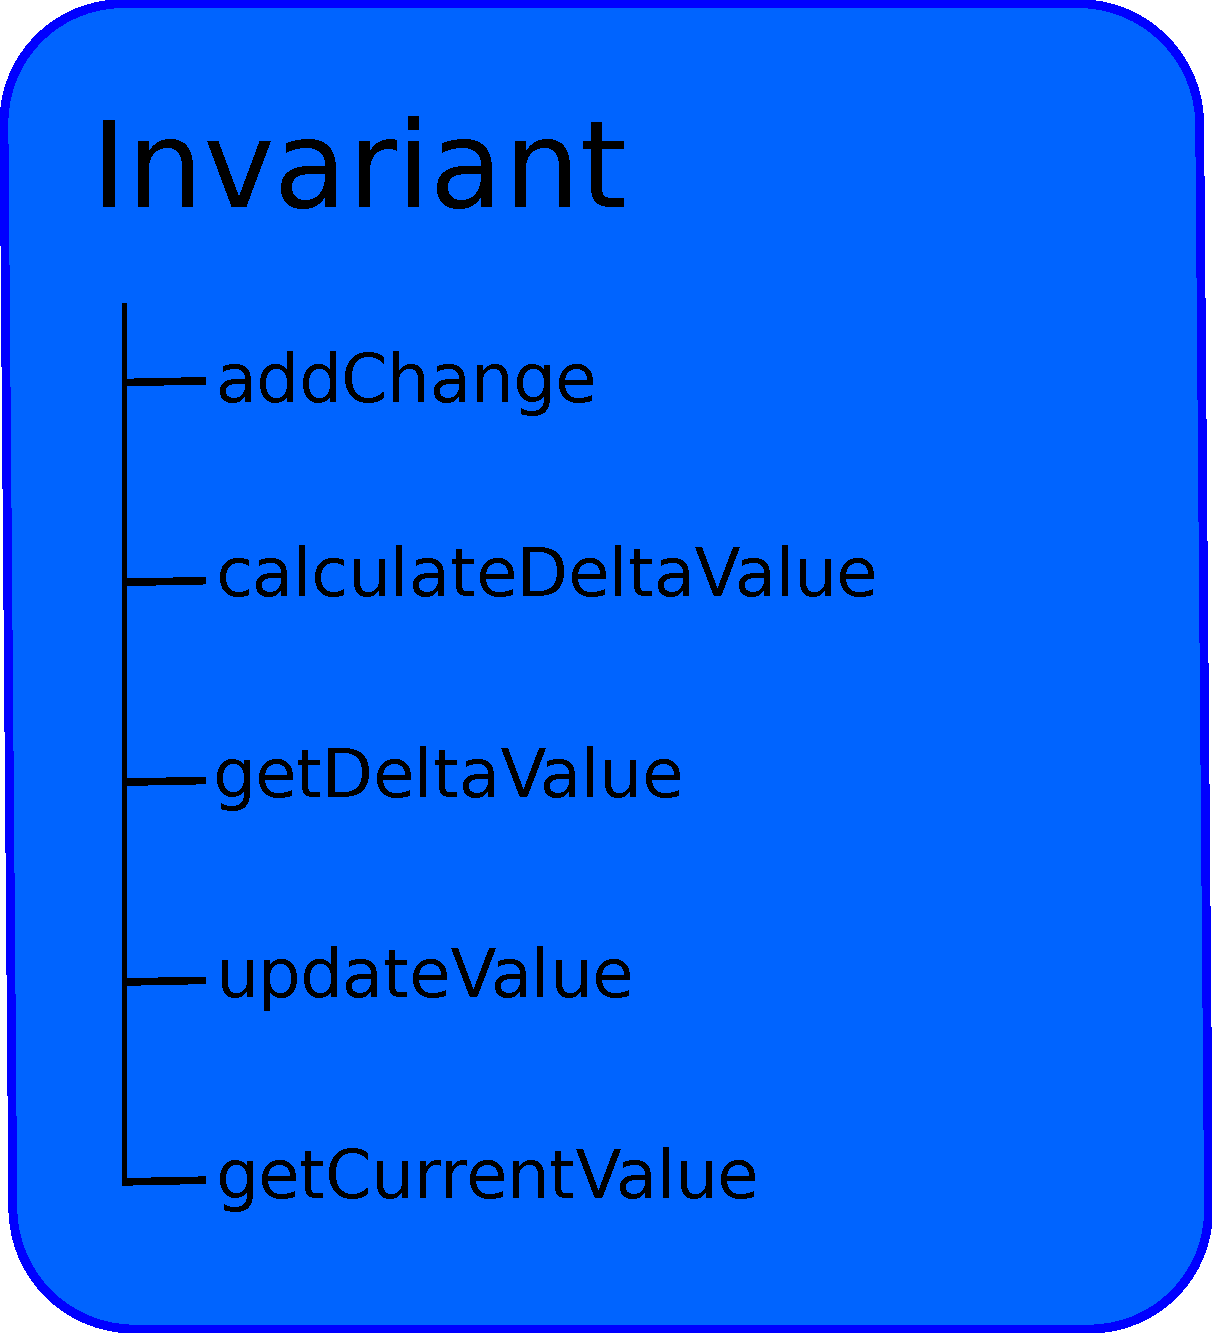
\includegraphics[width=\linewidth/2]{invariant.pdf} \caption{Important methods in Invariant 
class}\label{fig_invariant}
\end{center} 
\end{figure}
Invariants are only introduced after an initial solution to an instance is found and before the local 
search has begun. Invariants can represent either a variable or an auxiliary variable and are defined by oneway 
constraints. All Invariants must implement the methods \method{addChange}, \method{calculateDelta}, and 
\method{updateValue} that are used during local search. The \method{addChange} is used to tell an invariant that a 
variable in the oneway constraint defining it has been changed. The \method{calculateDelta} is used by the delta 
evaluation function in local search and updates the delta value of the invariant according to the changes 
received from \method{addChange}. The method \method{updateValue} is called when a move is performed to update the 
calue of the invariant. \\ 
Each type of invariant must implement its own method since the methods can be different for each type of invariant. \\ 
Some of the classes created in the \class{Local Search Engine} uses invariants but do not differentiate between them. 
If invariants did not have a common parent class then each invariant type would need its own data structure for 
storage. Another benefit is the search procedures do not have to exam which invariants the model consist of since they 
all have the same methods. It also makes it easier to add new invariants since all the functionality is implemented by 
the new invariant and nothing has to be changed in the Local Search Engine. \\ 
 

